\section{Examples}
%<-------------------------------------------------------------------------->
More examples, with a street map, Dijkstra's algorithm and colorings, are
given in the next section (exercises of the French baccalaureate).

\subsection{Coloring with the Welsh--Powell algorithm}\label{sec:welsh}
An airline offers direct flights between the cities A, B, C, D, E, F and G.
In the graph below, the vertices are the cities and the edges are the
flights. Each airport receives a color, and two airports linked by a direct
flight must have different colors.

The vertices are sorted by decreasing degree; the first color goes to the
first vertex and to every following vertex not adjacent to a vertex of this
color, and so on.

\medskip
\begin{minipage}{7cm}
\begin{tikzpicture}
  \GraphInit[vstyle=Welsh]
  \tkzSetUpGraph[vertex line width=2pt]
  \Vertices[unit=2.5]{circle}{A,B,C,D,E,F,G}
  \Edges(G,E,F,G,B,D,E,C,D,A,C,B,A) \Edges(B,E)
\end{tikzpicture}
\end{minipage}
\hfill
\begin{minipage}{7cm}
\begin{tabular}{ccc}
\toprule
\itshape Vertex & \itshape Degree & \itshape Color\\
\midrule
B & $5$ & red\\
E & $5$ & blue\\
C & $4$ & green\\
D & $4$ & yellow\\
A & $3$ & blue\\
G & $3$ & green\\
F & $2$ & red\\
\bottomrule
\end{tabular}
\end{minipage}

\medskip
\begin{tkzexample}[latex=7cm,small]
\begin{tikzpicture}
  \GraphInit[vstyle=Welsh]
  \tkzSetUpGraph[vertex line width=2pt]
  \Vertices[unit=2.5]{circle}{A,B,C,D,E,F,G}
  \SetVertexNoLabel
  \AddVertexColor{red}{B,F}
  \AddVertexColor{blue}{E,A}
  \AddVertexColor{green}{C,G}
  \AddVertexColor{yellow}{D}
  \Edges(G,E,F,G,B,D,E,C,D,A,C,B,A)
  \Edges(B,E)
\end{tikzpicture}
\end{tkzexample}

The graph contains the complete subgraph $\{B,C,D,E\}$ of order 4: four
colors are necessary and the chromatic number is 4.

\newpage
\subsection{Dijkstra's algorithm}
The shortest path from the vertex $E$ to the vertex $S$.

\begin{tkzexample}[vbox]
\begin{tikzpicture}
  \GraphInit[vstyle=Dijkstra]
  \Vertex{E}
  \Vertex[x=3,y=2]{A}  \Vertex[x=3,y=-2]{B}
  \Vertex[x=7,y=-2]{C} \Vertex[x=7,y=2]{D}
  \Vertex[x=10,y=0]{S}
  \Edge[label=$3$](E)(A)
  \Edge[label=$1$](E)(B)
  \Edge[label=$1$](A)(B)
  \Edge[label=$3$](B)(C)
  \Edge[label=$3$,style={pos=.25}](A)(C)
  \Edge[label=$5$,style={pos=.75}](B)(D)
  \Edge[label=$4$](A)(D)
  \Edge[label=$1$](S)(D)
  \Edge[label=$3$](C)(S)
  \Edge[label=$1$](C)(D)
  \tkzHighlightPath[color=red,lw=2pt,style={opacity=.4}]{E,B,C,D,S}
\end{tikzpicture}
\end{tkzexample}

\def\ry{$\vrule width 5pt$}
\def\iy{$\infty$}
\vbox{\tabskip=0pt \offinterlineskip
\def\tablerule{\noalign{\hskip\tabskip\hrule}}
\halign to \hsize{\strut#&\vrule # \tabskip=0.6em plus8em&
\hfil#\hfil& \vrule#&
\hfil#\hfil& \vrule#&
\hfil#\hfil& \vrule#&
\hfil#\hfil& \vrule#&
\hfil#\hfil& \vrule#&
\hfil#\hfil& \vrule#&
\hfil#\hfil& \vrule#\tabskip=0pt\cr\tablerule
&& $E$ &&  $A$   &&  $B$   &&   $C$  &&  $D$   && $S$    && Choice  &\cr\tablerule
&& $0$ && \iy    && \iy    && \iy    && \iy    && \iy    && $E$     &\cr\tablerule
&& \ry && $3(E)$ && $1(E)$ && \iy    && \iy    && \iy    && $B$     &\cr\tablerule
&& \ry && $2(B)$ && \ry    && $4(B)$ && $6(B)$ && \iy    && $A$     &\cr\tablerule
&& \ry && \ry    && \ry    && $4(B)$ && $6(B)$ && \iy    && $C$     &\cr\tablerule
&& \ry && \ry    && \ry    && \ry    && $5(C)$ && $7(C)$ && $D$     &\cr\tablerule
&& \ry && \ry    && \ry    && \ry    && \ry    && $6(D)$ && $S$     &\cr\tablerule}}

\medskip
The shortest path is $EBCDS$, of length $6$.

\newpage
\subsection{Classic graphs with \tkzname{tkz-berge}}
\tkzname{tkz-berge} draws the classic graphs of graph theory with
\tkzname{tkz-graph}; all the macros and styles of this documentation apply.

\begin{tkzexample}[vbox,small]
\begin{tikzpicture}[scale=.7]
  \GraphInit[vstyle=Art]
  \grPetersen[RA=2.5,RB=1.2]
  \begin{scope}[xshift=7cm]
    \grHypercube[RA=1.8]{4}
  \end{scope}
  \begin{scope}[xshift=14cm,yshift=2cm]
    \grTree[RA=.7,RB=1.4]{3}{2}
  \end{scope}
\end{tikzpicture}
\end{tkzexample}

\endinput
